\documentclass[crop=true]{standalone}
\usepackage{tikz}
\usepackage{tkz-euclide}

\begin{document}

% 全体集合$U$を$U={1,2,3,4,5}$とし, 部分集合$A,B$を$A = {1, 2, 3}, B = {3, 4}とする

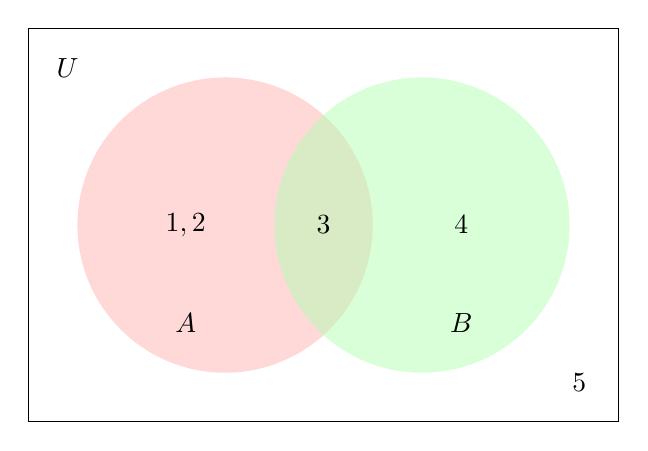
\begin{tikzpicture}[scale=2.5]

	\draw (-1.5, 1)--(-1.5, -1)--(1.5,-1)--(1.5, 1)--cycle;
	\begin{scope}[opacity=0.5]
	    \fill[red!30!white]   (0:-.5) circle (.75);
	    \fill[green!30!white] (0:.5) circle (.75);
	\end{scope}
    
    \node at(-.7, -.5) {$A$};
    \node at(.7, -.5) {$B$};
    \node at(-1.3, 0.8) {$U$};
    \node at(0:-.7) {$1, 2$};
    \node at(0,0) {$3$};
    \node at(0:.7) {$4$};
    \node at(1.3, -0.8) {$5$};

\end{tikzpicture}

\end{document}
